\documentclass{article}

\usepackage{amsmath}
\usepackage{url}
\usepackage{graphicx}
\usepackage{float}
\usepackage{amsthm}
\usepackage[a4paper, margin=1in]{geometry}
\usepackage{amssymb}
\usepackage{enumerate}

\theoremstyle{definition}
\newtheorem{definition}{Definition}[section]
\newtheorem{problem}{Problem}
\newtheorem{example}{Example}[section]

\theoremstyle{plain}
\newtheorem{theorem}{Theorem}[section]
\newtheorem{lemma}{Lemma}[section]
\newtheorem{corollary}{Corollary}[theorem]

\theoremstyle{remark}
\newtheorem*{remark}{Remark}

\renewcommand{\Re}{\operatorname{Re}}
\renewcommand{\Im}{\operatorname{Im}}
\newcommand{\reals}{\mathbb{R}}

\title{Characteristic Functions}
\author{Fu Tianwen \and Yao Chaorui \and Zhao Feng}

\begin{document}
\maketitle
\section{Sum of Two Independent Random Variable}
Let's consider the following problems:
\begin{problem}
	Rain falls on your head at $\lambda$ drops per second on average. What is the distribution of rain drops on your head in two seconds?
	\label{prb:poisson}
\end{problem}
\begin{problem}
	$X_1\sim N(\mu_1,\sigma_1^2), X_2\sim N(\mu_2,\sigma_2^2).$ $X_1,X_2$ are independent. Distribution of $Y=X_1+X_2$?
	\label{prb:normal}
\end{problem}
\noindent With what we have already learned, it is really easy to calculate the statistics(expectation, variance, ...) of the sums. But what is the distribution? Are they the same as the parts or some strange distribution?
One may suggest calculating them by convolution. But is there some simpler idea?
That leads to the topic we're going to talk about today -- characteristic functions.
\section{Characteristic Functions}
\subsection{Definition}
\begin{definition}
	Let $X$ be a random variable and denote by $F$ the cumulative distribution function of $X$ (or $f$ the probability density function). The characteristic function $\varphi=\varphi_X$ of $X$ (or of $F$, in which case we also write $\varphi_F$) is defined by \cite{cfms}
	$$\varphi_X(t):=E[e^{itX}]=\int_{-\infty}^\infty e^{itx}dF(x)=\int_{-\infty}^\infty e^{itx}f(x)dx, t\in\reals$$
\end{definition}
\noindent The $i$ mentioned above is the imaginary unit. If you have no knowledge of complex numbers, all you need to know is simply:
\begin{enumerate}[$\ast$]
	\item $i^2=-1$,
	\item $e^{i\theta} = \cos\theta + i\sin\theta$. (This formula comes from Taylor Series)
\end{enumerate}
\subsection{Properties}
\begin{theorem}[Uniqueness Theorem \cite{uChicago}]
	Let $X$ be a real random variable with distribution function
	$F$ and characteristic function $\varphi$. Similarly, let $Y$ have distribution
	function $G$ and characteristic function $\psi$. If $\varphi(t) = \psi(t)$ for all $t\in\reals$
	then $F(x) = G(x)$ for all $x \in\reals$.
\end{theorem}
\begin{remark}
	From this we may easily conclude the distribution of a random variable if we can prove that its characteristic function is of the same form as a known distribution.
\end{remark}
\begin{theorem}[Inversion Formula \cite{pte}]
If $\int_\reals |\varphi(t)| dt < \infty$ then $X$ has bounded continuous density
$$
f(x) = \frac1{2\pi} \int e^{-itx}\varphi(t)dt
$$

\end{theorem}
\begin{theorem}
	If $X$ and $Y$ are independent random variables then the characteristic function of their sum is\footnote{Properties \ref{thm:indept} and \ref{thm:linear} on come from Bisgaard and Zoltan's book \cite{cfms}.} 
	$$\varphi_{X+Y}(t) = \varphi_{X}\cdot\varphi_{Y}.$$
	\label{thm:indept}
\end{theorem}
\begin{remark}
This gives us a much simpler way than convolution.
\end{remark} 
\begin{remark}
If $X$ and $Y$ are random variables such that $\varphi_{X+Y} = \varphi_X\cdot\varphi_Y $, then in general we do not conclude $X$ and $Y$ are independent. (See page 13 in \cite{cfms})
\end{remark} 
\begin{corollary}
	The product of two characteristic functions is a characteristic function.
\end{corollary}
\begin{theorem}
	For any $a,b \in \reals$, $$\varphi_{aX+b}(t)=e^{ibt}\varphi_X(at).$$
	\label{thm:linear}
\end{theorem}
\subsection{Common Distributions and Their Characteristic Functions}
First we try to derive the characteristic function for $X\sim Exponential(\lambda)$.
Then
$$
\begin{aligned}[t]
\varphi_X(t) &:=E[e^{itX}] &\\
&=\int_{-\infty}^\infty e^{itx}f(x)dx & \\
&=\int_0^\infty e^{itx}\cdot \lambda e^{-\lambda x}dx & \text{By distribution of x} \\
&=\frac{\lambda}{it-\lambda}e^{(it-\lambda)x} \bigg|_0^\infty & \\
&=\frac{\lambda}{\lambda-it} & \text{By Squeeze Theorem}
\end{aligned}
$$
where the last two steps can be justified by
$$\lim\limits_{x\to\infty}|e^{(it-\lambda)x}| = \lim\limits_{x\to\infty}|e^{-\lambda x}|
=0 \text{ for positive }\lambda$$
Characteristic functions of other distributions can be seen in table \ref{tbl:charFunc}.
\begin{table}[ht]
	\caption{Characteristic Functions for Common Distributions\cite{kurser}}
	\centering
	\begin{tabular}{l l l}
		\hline\hline
		Distribution  & PMF/PDF & Characteristic Function\\
		\hline
		Constant $X\equiv a$  & - &  $\varphi_X(t) = e^{iat}.$\\
		Binomial $X\sim Binomial(m,p)$ & $p_X(n) = \binom{n}{m} p^n(1-p)^{m-n}$ &
		$\varphi_X(t) = (pe^{it} + (1-p))^m$\\
		Poisson $X\sim Poisson(\lambda)$ & $p_X(n) = \frac{\lambda ^n}{n!} e^{-\lambda}$ &
		$ \varphi_X(t)=e^{\lambda(e^{it}-1)} $\\
		Exponential $X \sim Exponential(\lambda)$ & $p_X(n) = \lambda e^{-\lambda x}$ &
		$\varphi_X(t)=\frac{\lambda}{\lambda-it}$ \\
		Normal $X\sim N(0,1)$ & $f_X(x) = \frac{1}{\sqrt{2\pi}}e^{-\frac{x^2}{2}}$ &
		$\varphi_X(t)=e^{-\frac{t^2}{2}}$\\
		Normal $Y\sim N(\mu,\sigma ^2)$ & $f_Y(y) = \frac{1}{\sqrt{2\pi}\sigma}e^{-\frac{(y-\mu)^2}{2\sigma ^2}}$ & $\varphi_Y(t)=e^{it\mu-\frac{\sigma^2 t^2}{2}}$
	\end{tabular}
	\label{tbl:charFunc}
\end{table}
\subsection{Bridge between Probability and Statistics}
So what "characteristics" are these weird "characteristic functions" talking about? To understand this, first we need some knowledge about \textbf{moments}.
\begin{definition}[Moment \cite{wiki:moment}]
For probability density functions $f$ (or cumulative density function $F$), the moments are given by
$$\mu_n' = E[X^n] = \int_{-\infty}^\infty x^ndF(x) = \int_{-\infty}^\infty x^nf(x)dx $$
\end{definition}
\begin{remark}
Not to be confused with mean $\mu$. 
\end{remark}
\noindent\textbf{Relation with statistics.} Observe that the first moment is simply the expectation. The second moment is related to the variance: $Var[X]=E[X^2]-(E[X])^2$. What about the third moment? A related concept is \textbf{skewness}\cite{wiki:skewness}:
\begin{figure}[H]
	\centering
	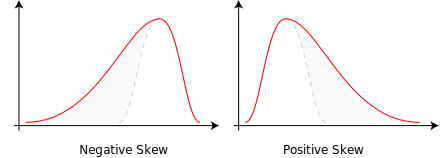
\includegraphics[width=0.8\linewidth]{img/Negative_and_positive_skew_diagrams_(English)}
	\caption{Two distributions with the same expectation and variance, but different skewness} 
	\label{fig:skewness}
\end{figure}
\noindent Now let's consider the values of derivatives of $\varphi_X(t)$ at 0:
$$
\begin{aligned}[t]
&\varphi_X(t)=\int_{-\infty}^\infty e^{itx}f(x)dx; & \varphi_X(0)=1\\
&\varphi'_X(t)=i\int_{-\infty}^\infty xe^{itx}f(x)dx; & \varphi'_X(0)=iE[X]\\
&\varphi''_X(t)=i^2\int_{-\infty}^\infty x^2e^{itx}f(x)dx; & \varphi''_X(0)=i^2E[X^2]\\
&\cdots
\end{aligned}
$$
\noindent By simple induction one can get the following:
\begin{theorem}
	Suppose $X$ is a random variable for which the $n$th moment exists. Suppose $\varphi_X(t)$ is the characteristic function of $X$, and $\varphi_X(t)$ is $n$-times differentiable. Then the $n$th moment $$E[X^n]=i^{-n}\biggl[\frac{d^n}{dt^n}\varphi_X(t)\biggr]_{t=0}$$
\end{theorem}
\noindent\textbf{Therefore with infinite statistics we may reconstruct the distribution by characteristic functions.}\\
\section{Solutions to the Problems}
With the powerful characteristic functions, the sums of independent random variables are just a piece of cake.\\
\noindent\textbf{Solution to Problem \ref{prb:poisson}.}
Our intuition tells us that it should be $Poisson(2\lambda)$. \\
Let $X,Y$ be two independent $Poisson(\lambda)$ random variables. Let $Z=X+Y$.
Notice that characteristic functions for $X$ (and respectively $Y$) is $\varphi_X(t)=e^{\lambda(e^{it}-1)}$.
Therefore we have $\varphi_Z(t)=\varphi_{X+Y}(t)=(\varphi_X(t))^2=e^{2\lambda(e^{it}-1)}$. 
By uniqueness of characteristic functions we know that $Z\sim Poisson(2\lambda)$.
\begin{remark}
	By similar ideas, one can show that the sum of two independent poisson random variables has a possion distribution with an expectation of the sum of both expectations.
\end{remark} 
\noindent\textbf{Solution to Problem \ref{prb:normal}.}
Similarly to previous problem $$\varphi_{Y}(t)=\varphi_{X_1+X_2}(t)=e^{it\mu_1-\frac{\sigma_1^2 t^2}{2}}\cdot e^{it\mu_2-\frac{\sigma_2^2 t^2}{2}}$$
Therefore we have $$\varphi_Y(t)=e^{it(\mu_1+\mu_2)-\frac{(\sigma_1^2+\sigma_2^2)t^2}{2}}$$
which implies that $Y\sim N(\mu_1+\mu_2,\sigma_1^2+\sigma_2^2)$
\begin{remark}
	This shows that the sum of two independent normal random variables is another normal random variable, the mean and standard deviation of which is the same as calculated statistically from the two components. 
\end{remark}
\section{Other Examples}
\begin{example}
	Show that $Poisson(\lambda)$ is the same as $\lim\limits_{n\to\infty}Binomial(n,\frac{\lambda}{n})$.
\end{example}
\noindent\textbf{Solution.}
Take the limit of the characteristic function of the binomial distribution.
$$\begin{aligned}
\lim\limits_{n\to\infty}\varphi_B(t)&
=\lim\limits_{n\to\infty}(\frac{\lambda}{n}e^{it}+(1-\frac{\lambda}{n}))^n\\
&=\lim\limits_{n\to\infty}(1+(e^{it}-1)\frac{\lambda}{n})^n\\
&=e^{\lambda(e^{it}-1)}
\end{aligned}$$
\begin{remark}
	This is not a standard way of defining Poisson distribution; however, this gives us a nice intuition of Poisson distribution and can be seen as a proof for the formula of the characteristic function of it.
\end{remark}
\section{Central Limit Theorem}
First we prove a useful lemma\footnote{The proofs for lemma \ref{lem:clt} and theorem \ref{thm:clt} are not rigorous and serves only for intuitively demonstrating the usage of Characteristic Functions. See the references\cite{waterloo,nus} for detailed proofs.}:
\begin{lemma}
	For any random variable $X$ with $E[X]=0,Var[X]=1$, we have $\varphi_X(t)=1-\frac12t^2+o(t^2)$.
	\label{lem:clt}
\end{lemma}
\begin{proof}
	Directly from the definition and Taylor Series we have
	$$\varphi_X(t)=E[e^{itX}]=E[1+itX+\frac12i^2t^2X^2+o((tX)^2)]$$
	By linearity of expectation,
	$$\varphi_X(t)=E[1]+itE[X]-\frac12t^2E[X^2]+o(t^2)$$
	Also
	$$E[X^2]=Var[X]-(E[X])^2=1$$
	Therefore $$\varphi_X(t)=1-\frac12t^2+o(t^2)$$
\end{proof}
\begin{theorem}[Central Limit Theorem\cite{waterloo}]
	If $X_i$ are independent identically distributed random variables with $E[X_i] = \mu, Var[X_i] = \sigma^2$ , then $S_n^* = \frac1{\sigma\sqrt n}\sum_{i=1}^n(X_i-\mu)$ converges weakly to $N(0, 1)$.
	\label{thm:clt}
\end{theorem}
\begin{remark}
	Note that theorem \ref{thm:clt} is equivalent to the one given in class.
\end{remark}
\begin{proof}
	By Lemma \ref{lem:clt} we denote the characteristic function of $\frac{X_i-\mu}{\sigma}$ by $\varphi(t)$, then  $\varphi(t)=1-\frac12t^2+o(t^2)$. Therefore the characteristic function of $S_n^*$ is 
	$$\varphi^n(t/\sqrt{n})=[1-\frac{t^2}{2n}+o(t^2/n)]^n$$
	Take $n\to\infty$ and we get the characteristic function of $\lim\limits_{n\to\infty}S^*_n$
	$$\varPhi(t)=\lim\limits_{n\to\infty}\varphi^n(t/\sqrt{n})
	=\lim\limits_{n\to\infty}[1-\frac{t^2}{2n}]^n=e^{-\frac{t^2}2}$$
	Therefore $\lim\limits_{n\to\infty}S_n^*$ converges to $N(0,1)$.
\end{proof}
\medskip

\bibliographystyle{ieeetr}
\bibliography{bibliography}
\end{document}
